\section{Solution}
Our description of our solution will be rooted in two major parts, as described in the introduction.
The following part regards our texture mapping and morphology.\newline

\subsection{Floor Tracking}
To get in touch with the concepts of morphology, our first assignment was to map the path of a person described by a video file. This mapping should be done, such that the path would correctly appear on an actual map.\newline

The videofile we were provided came accompanied by data related to the movement of the person.\newline

Solving this assignment required us to create the function \textsl{DisplayTrace(...)}, which processes the data and draws the trace onto the actual map. This function draws upon some properties of the \textsl{showFloorTrackingData()} function, and by its extension the \textsl{getHomographyFromMouse(...)} function.\newline

In the \textsl{DisplayTrace(img, points, H)} function we start out by going through all points provided by the list "points". These are created in the \textsl{showFloorTrackingData()} function, so we start our research there.\newline

The \textsl{showFloorTrackingData()} function finds the three boxes that contain the person which we are tasked to track. Each box determains a different part of the person; red is upper body, blue is complete body, and green is lower body. As such, we have chosen to track the "green box", which is the box that describes the feet of our target.
The feet should be the best point to go for, since it will be the most precise. Should the camera have a very sharp angle of attack, plotting from the face or torso could give very unaccurate results. The homography will be created such that the floor coordinates get malformed.\newline

\begin{figure}
	\centering
	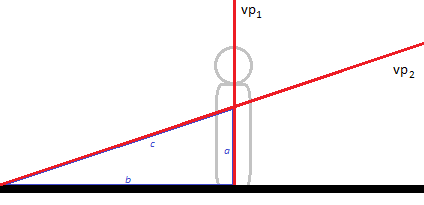
\includegraphics[scale=0.9]{images/viewpointdifference.png}
	\caption{Differences in viewpoints.}
	\label{fig:viewpoints}
\end{figure}

Looking at figure \ref{fig:viewpoints}, we can tell that the difference between the two points \(p1,p2\) on the base plane represented by \(vp_1\) is \(b_l\) when the angle of attack on \(vp_2\) is sharpened. The difference \(b_l\) is dependant on \(a_l\), given that \(b_l = \sqrt{c_l^2-a_l^2}\). \(c_l = \frac{a_l}{sin(A)}\)\newline

We have chosen the bottom middle spot of the green box, to avoid these complications. This should be the most precise point when considering its proximity to the ground, along with its position horizontally. Given the green box \(B_(x,y,w,h)\), we can find the best point \(p_(x,y)\) with the following calculations:
\[p_y = B_y+B_h \quad | \quad p_x = B_x + (B_w / 2)\]

Now that we have our point, we need to transfer it into a valid point on our map. We do this using a homography.

A homography has the interesting ability, that it is capable of turning one set of coordinates into another. This way, we can insert the coordinates of our traced pathing, and it will help us translate them to fit the map.

With the traced path in hand and translated, we can go paint the path onto the map, in our case, something that is done with the CV2 library and its \textsl{cv2.circle(...)} function.

\subsection{Texture Mapping}

\subsection{Camera Calibration}
With this subsection we start the second part of the assignment. With the help of an updated version of the \textsl{SIGB-Tools2.py} library the first task was to start learning the different functionalities of the file \textsl{Assignment_Cube.py}. Once we got to know the code we began with the camera calibration. For this task we used the \textsl{calibrateCamera} function in our tools library and a printed chessboard of size 6x9. This function uses several important variables like \textsl{pattern_points}, \textsl{img_points}, and \textsl{img_points_first}.  \textsl{Pattern_points} are the position of the inner points of the chessboard squares in the calibration pattern coordinate space. \textsl{Image_points} are the corners of the chessboard found in the image being captured by the webcam and  \textsl{image_points_first} contains the \textsl{image_points} for a picture taken in the first frame of the video. 
The calibration is done by taking 5 sample views and saves information like the camera calibration matrix, rotation vectors and translation vectors. By modifying the number of samples taken by the calibration function we noticed that increasing the number of samples also increases the accuracy of the calibration and viceversa.\newline 
After calibrating the camera the next step was to calculate the camera matrix  \textsl{ \(P_1\) = K[ \(R_1\)| \(t_1\) ]} for the first view. This camera matrix with its rotation and translation vectors helped us to project the points taken from the chessboard pattern during the calibration of the camera onto the first view image as seen in figure \ref{fig:projection}. 
\begin{figure}
	\centering
	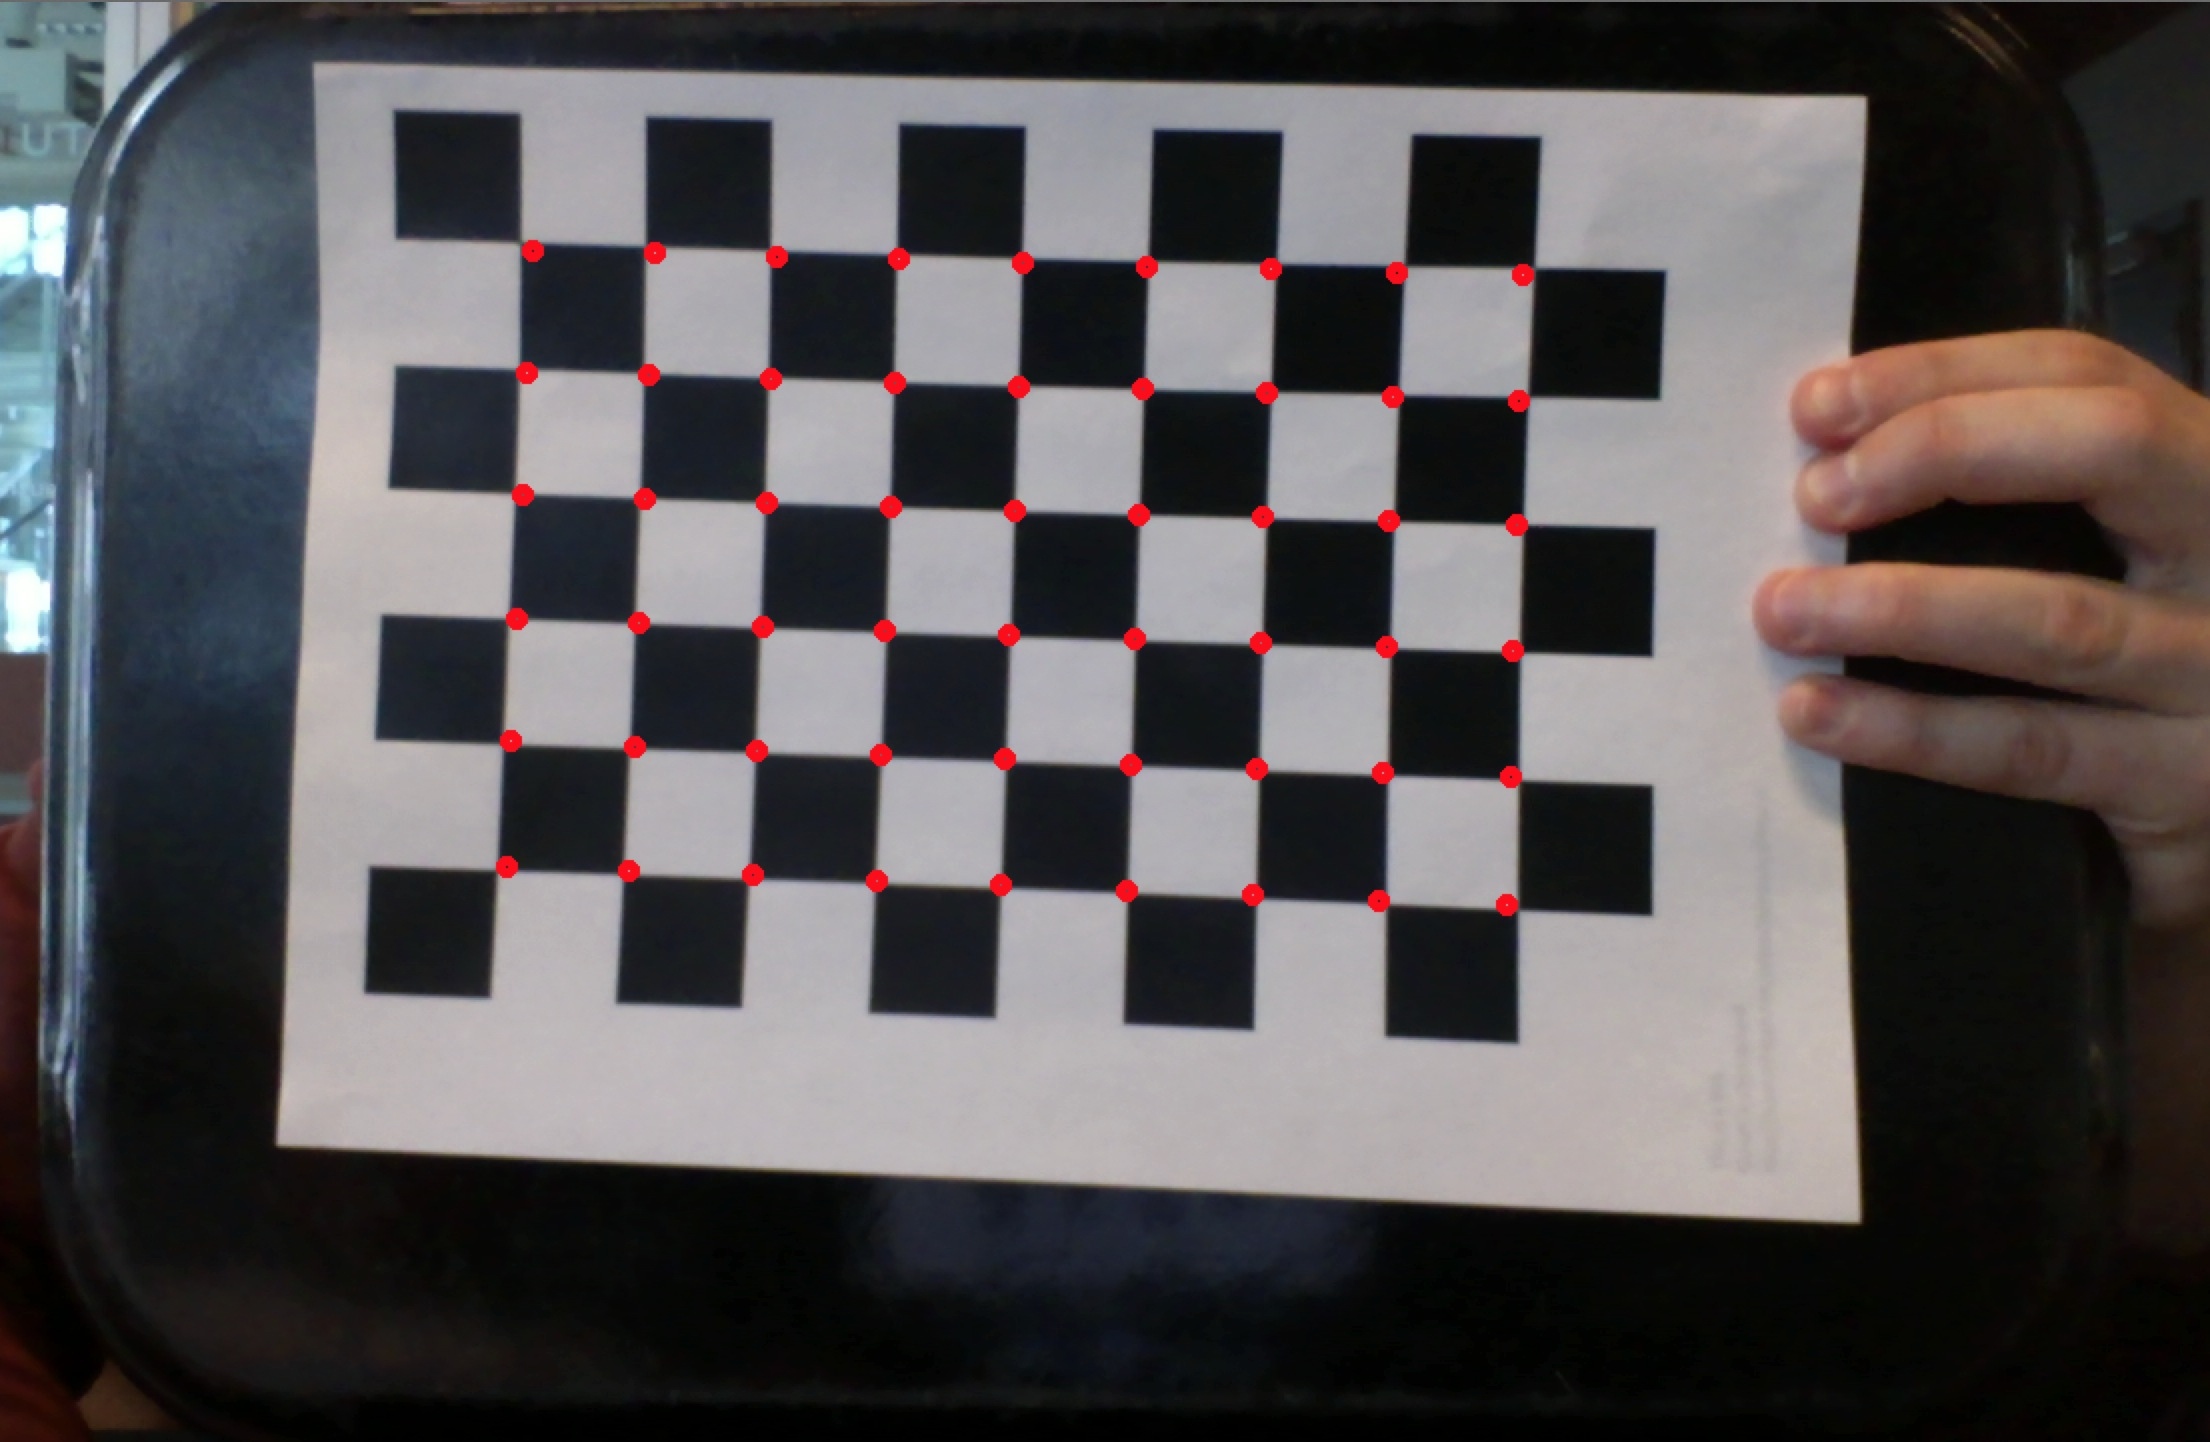
\includegraphics[scale=0.9]{images/projection_p1.jpg}
	\caption{Projection of chessboard pattern points to first view image}
	\label{fig:projection}
\end{figure}

\subsection{Augmentation}
For the augmentation part in this assignment the goal is to calculate the camera matrix in each video frame taken from the webcam and project a 3D cube to the same view. The camera matrix is calculated using two different methods: through homographies and directly using extrinsic parameters. \newline
In the first method two Homographies where used. The first Homography is from the chessboard calibration pattern to the first view image, \(H_cp-fv\). The second Homography is from the first view image to the current view image from the webcam, \(H_fv-cv\). In order to get the second homography we had to locate the 4 outer corners of the calibration patter in the playing video. Having these two homographies we could compute the homograph form the chessboard pattern to the current view of the webcam by applying a dot product which gave us the homography \(H_cp-cv\). This third homography was used to calculate the camera matrix \textsl{P2_Method1}. Several operations had to be applied to get to this result. First, the previous camera matrix was broken apart to get the intrinsic parameters' matrix \textsl{K} which were used to compute the new rotation vector. Second, a dot product between the previous camera matrix and the homography \(H_cp-cv\) was applied and the result was complemented with the new rotation vector to conform the new camera matrix \textsl{P2_Method1}.\newline
The second method uses the function \textsl{GetIObjectPos()} located in our tools library. This function finds the object pose from 3D-2D point correspondences and returns new rotation and translation vectors. The points used for this method are \textsl{obj_points} used in the first part and the corners of the current view from the webcam. The new vectors computed by this function are combined and multiplied by dot product with the previous camera matrix to compute the new \textsl{P2_method2} camera matrix.
\begin{figure}
	\centering
	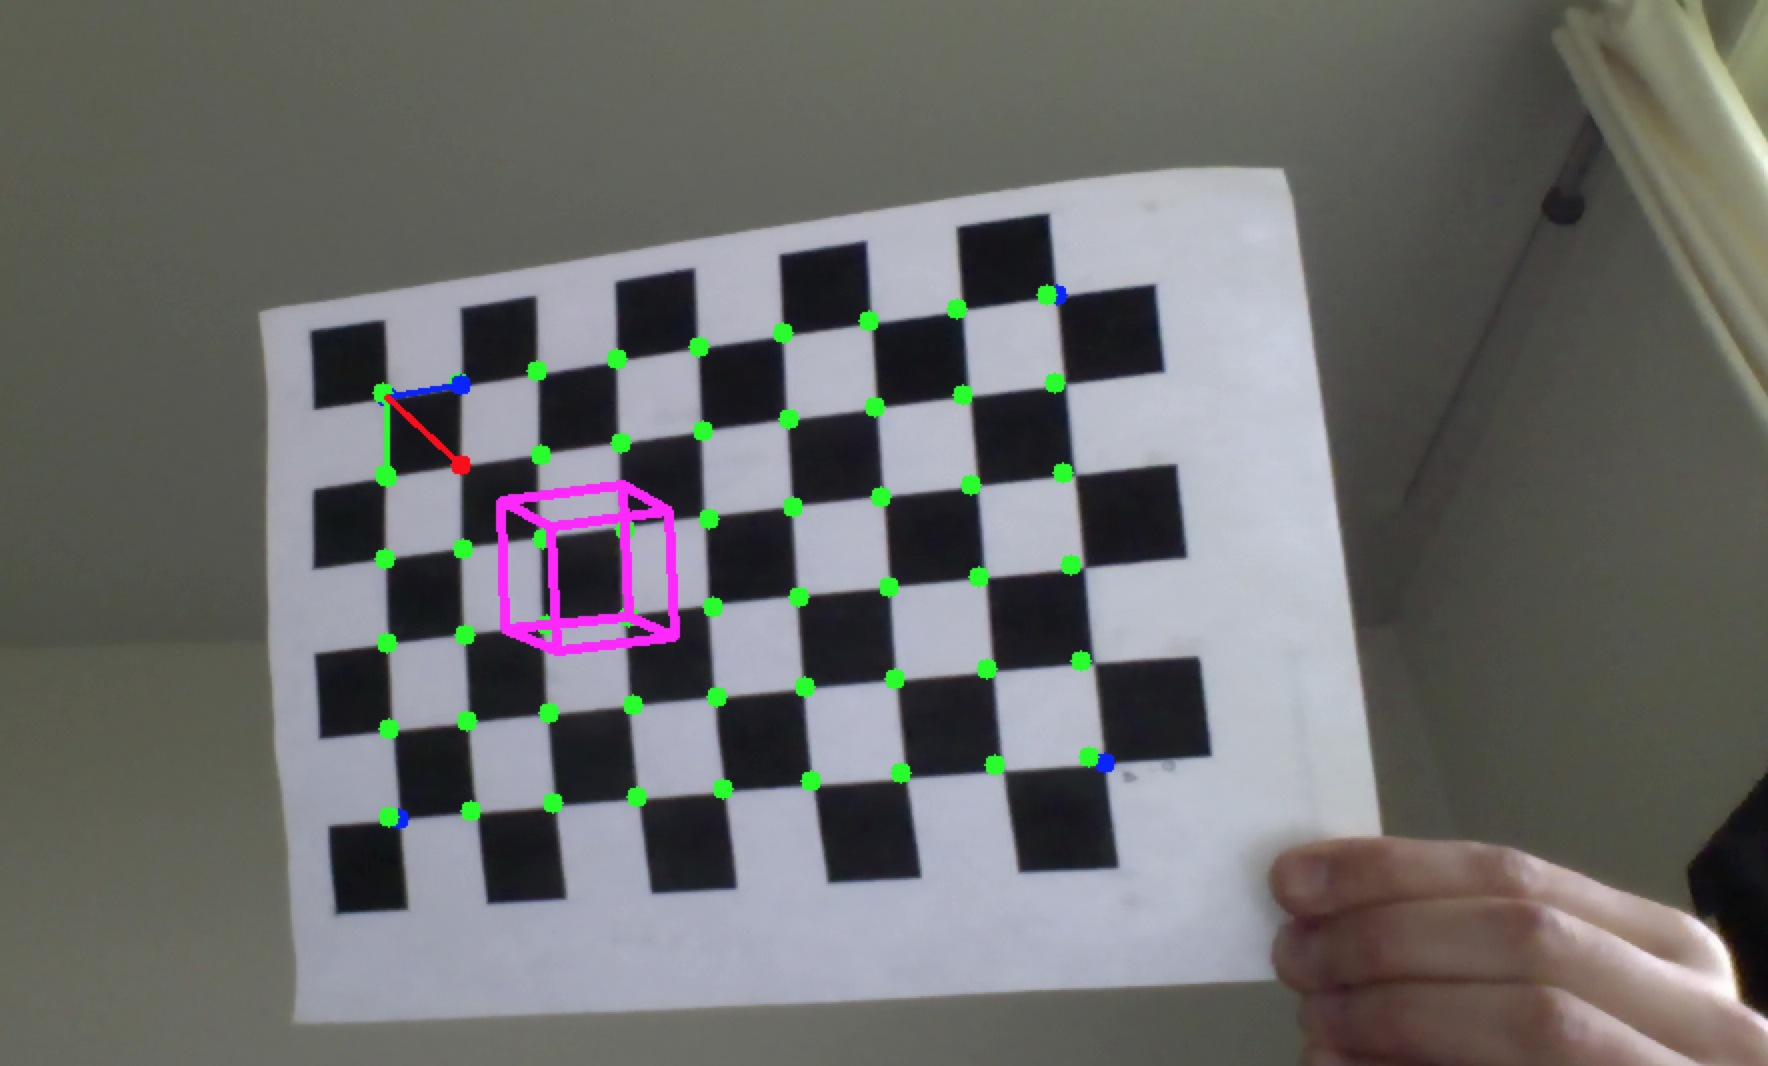
\includegraphics[scale=0.9]{images/p2_method2.jpg}
	\caption{Projection of chessboard pattern points to webcam feed with P2_method2}
	\label{fig:method2}
\end{figure}

After finding the new camera matrices we proceed to draw the world coordinate axes in the chessboard pattern and project the 3D cube as seen in \ref{fig:method2}.\newline
Comparing the two camera matrices and their respective projections we come to the conclusion that the camera matrix \textsl{P2_method2} has a better performance than \textsl{P2_method1}. 	

